\section{ Unfolded Differential Cross-sections }
\label{sec:DifferentialxS}

The background-subtracted data is unfolded using the iterative Bayesian Unfolding discussed in Section \ref{sec:Unfolding}. The unfolded differential cross-sections, the main results of this thesis, are obtained by multiplying the inverse of the integrated luminosity to the background-subtracted unfolded yield in each bin. The unfolded differential cross-section for eleven kinematic observables is shown in Figures \ref{fig:unfolded_xs_VBS_Enhanced_a} and \ref{fig:unfolded_xs_VBS_Enhanced_b}. 

Each distribution of unfolded differential cross-section is compared to two different state-of-the-art particle-level SM predictions, one in which the QCD $qqZZjj$ contribution is predicted by the \textsc{Sherpa} generator, and the other where the QCD $qqZZjj$ contribution is predicted by \textsc{Madgraph} generator. The light-red and light-blue bands are the fiducial level systematics on the \textsc{Sherpa} and \textsc{Madgraph} particle-level cross-sections, respectively. The vertical error bars on the unfolded cross-section are the statistical uncertainty. In contrast, the black band represents the total systematic uncertainties on unfolded cross-sections from theoretical, experimental, and unfolding sources. The unfolded cross-sections are limited by statistical precision in all distributions and all bins. For some distributions, one or two events are found in the overflow bin resulting from bin migrations. These events are added to the content of the last bin of the unfolded distribution. 

Generally, for all distributions, the data is well modeled by the MC simulations within $2\sigma$ of the uncertainty band. Two p-values are determined by comparing unfolded cross-sections to the two predicted cross-sections to quantify the agreement between the experimentally measured unfolded data and the SM-predicted cross-sections. The p-values are calculated based on a technique discussed in Ref\cite{pValueStat} by taking the residual and uncertainties of two weighted histograms. For all kinematic observables, the reported p-values obtained by comparing to either generator are more significant than $0.05$. Therefore, in the analyzed LHC Run-2 dataset, for the $ZZ^*(\rightarrow 4 \ell) jj$ process, all differential cross-sections in the VBS-Enhanced region are concluded to agree with the SM predictions. 

\begin{figure}[!htb]
    \centering
    \begin{subfigure}{.48\textwidth}
        \centering
        \includegraphics[width=.98\linewidth]{figures/Results/CrossSection_VBSEnhanced/xs_mjj_SR.pdf}
        \caption{ \footnotesize{$m_{jj}$: p-value (Sherpa=0.95 $\&$ MG=0.91)}}
    \end{subfigure}
    \begin{subfigure}{.48\textwidth}
        \centering
        \includegraphics[width=.98\linewidth]{figures/Results/CrossSection_VBSEnhanced/xs_m4l_SR.pdf}
        \caption{ \footnotesize{$m_{4\ell}$: p-value (Sherpa=0.84 $\&$ MG=0.45)} }
    \end{subfigure}\\
    \begin{subfigure}{.48\textwidth}
        \centering
        \includegraphics[width=.98\linewidth]{figures/Results/CrossSection_VBSEnhanced/xs_ptjj_SR.pdf}
        \caption{ \footnotesize{$p_{T,jj}$: p-value (Sherpa=0.97 $\&$ MG=0.85)}}
    \end{subfigure}
    \begin{subfigure}{.48\textwidth}
        \centering
        \includegraphics[width=.98\linewidth]{figures/Results/CrossSection_VBSEnhanced/xs_pt4l_SR.pdf}
        \caption{ \footnotesize{$p_{T,4\ell}$: p-value (Sherpa=0.98 $\&$ MG=0.94)}}
    \end{subfigure}\\
    \begin{subfigure}{.48\textwidth}
        \centering
        \includegraphics[width=.98\linewidth]{figures/Results/CrossSection_VBSEnhanced/xs_ptzzjj_SR.pdf}
        \caption{ \footnotesize{$p_{T,4\ell jj}$: p-value (Sherpa=0.92 $\&$ MG=0.80)}}
    \end{subfigure}
    \begin{subfigure}{.48\textwidth}
        \centering
        \includegraphics[width=.98\linewidth]{figures/Results/CrossSection_VBSEnhanced/xs_stzzjj_SR.pdf}
        \caption{ \footnotesize{$s_{T, 4\ell jj}$: p-value (Sherpa=0.94 $\&$ MG=0.83)}}
    \end{subfigure}
    \caption{Unfolded differential cross-sections in the VBS-Enhanced region.} \label{fig:unfolded_xs_VBS_Enhanced_a}
\end{figure}

\begin{figure}[!htb]
    \centering
    \begin{subfigure}{.49\textwidth}
        \centering
        \includegraphics[width=.98\linewidth]{figures/Results/CrossSection_VBSEnhanced/xs_cosThetaStar1_SR.pdf}
        \caption{ \footnotesize{$\cos \theta^{*}_{\ell 1 \ell 2}$: p-value (Sherpa=0.80 $\&$ MG=0.55)}}
    \end{subfigure}
    \begin{subfigure}{.49\textwidth}
        \centering
        \includegraphics[width=.98\linewidth]{figures/Results/CrossSection_VBSEnhanced/xs_cosThetaStar3_SR.pdf}
        \caption{ \footnotesize{$\cos \theta^{*}_{\ell 3 \ell 4}$: p-value (Sherpa=0.71 $\&$ MG=0.30)} }
    \end{subfigure}\\
    \begin{subfigure}{.49\textwidth}
        \centering
        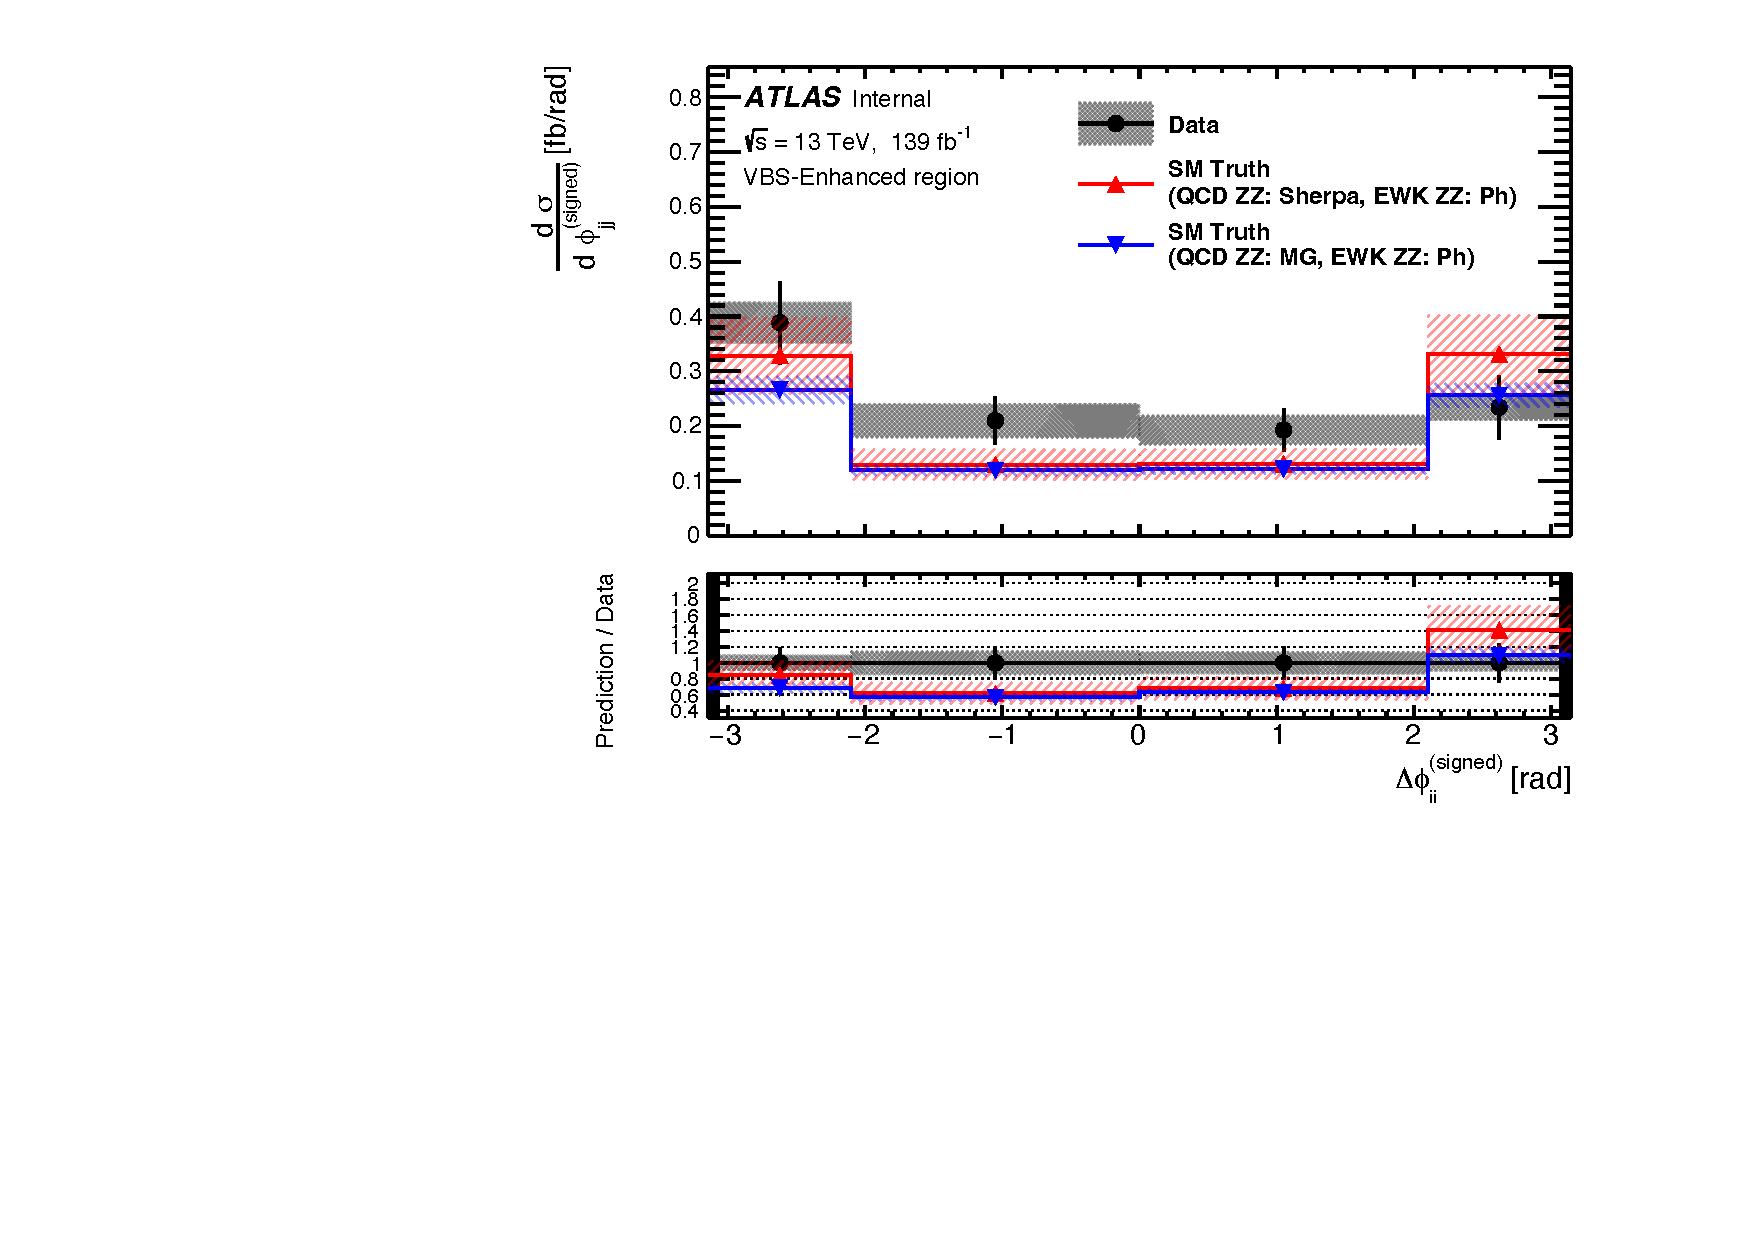
\includegraphics[width=.98\linewidth]{figures/Results/CrossSection_VBSEnhanced/xs_dphi_SR.pdf}
        \caption{ \footnotesize{$\Delta \phi _{jj}^{signed}$: p-value (Sherpa=0.28 $\&$ MG=0.18)} }
    \end{subfigure}
    \begin{subfigure}{.49\textwidth}
        \centering
        \includegraphics[width=.98\linewidth]{figures/Results/CrossSection_VBSEnhanced/xs_dy_SR.pdf}
        \caption{ \footnotesize{$\Delta y_{jj}$: p-value (Sherpa=0.96 $\&$ MG=0.93)} }
    \end{subfigure}\\
    \begin{subfigure}{.49\textwidth}
        \centering
        \includegraphics[width=.98\linewidth]{figures/Results/CrossSection_VBSEnhanced/xs_centrality_SR.pdf}
        \caption{ \footnotesize{$\zeta$: p-value (Sherpa=0.87 $\&$ MG=0.73)} }
    \end{subfigure}
    \caption{Unfolded differential cross-sections in the VBS-Enhanced region.}  \label{fig:unfolded_xs_VBS_Enhanced_b}
\end{figure}